\documentclass[]{article}
\usepackage{lmodern}
\usepackage{amssymb,amsmath}
\usepackage{ifxetex,ifluatex}
\usepackage{fixltx2e} % provides \textsubscript
\ifnum 0\ifxetex 1\fi\ifluatex 1\fi=0 % if pdftex
  \usepackage[T1]{fontenc}
  \usepackage[utf8]{inputenc}
\else % if luatex or xelatex
  \ifxetex
    \usepackage{mathspec}
  \else
    \usepackage{fontspec}
  \fi
  \defaultfontfeatures{Ligatures=TeX,Scale=MatchLowercase}
\fi
% use upquote if available, for straight quotes in verbatim environments
\IfFileExists{upquote.sty}{\usepackage{upquote}}{}
% use microtype if available
\IfFileExists{microtype.sty}{%
\usepackage{microtype}
\UseMicrotypeSet[protrusion]{basicmath} % disable protrusion for tt fonts
}{}
\usepackage[margin=1in]{geometry}
\usepackage{hyperref}
\hypersetup{unicode=true,
            pdftitle={Supplemental Materials \#3: Demonstration of the Incorrect Population Correlation Matrices and Model Specifications in Study 1 in Yu et al. (2016)},
            pdfauthor={Mike W.-L. Cheung},
            pdfborder={0 0 0},
            breaklinks=true}
\urlstyle{same}  % don't use monospace font for urls
\usepackage{color}
\usepackage{fancyvrb}
\newcommand{\VerbBar}{|}
\newcommand{\VERB}{\Verb[commandchars=\\\{\}]}
\DefineVerbatimEnvironment{Highlighting}{Verbatim}{commandchars=\\\{\}}
% Add ',fontsize=\small' for more characters per line
\usepackage{framed}
\definecolor{shadecolor}{RGB}{248,248,248}
\newenvironment{Shaded}{\begin{snugshade}}{\end{snugshade}}
\newcommand{\KeywordTok}[1]{\textcolor[rgb]{0.13,0.29,0.53}{\textbf{#1}}}
\newcommand{\DataTypeTok}[1]{\textcolor[rgb]{0.13,0.29,0.53}{#1}}
\newcommand{\DecValTok}[1]{\textcolor[rgb]{0.00,0.00,0.81}{#1}}
\newcommand{\BaseNTok}[1]{\textcolor[rgb]{0.00,0.00,0.81}{#1}}
\newcommand{\FloatTok}[1]{\textcolor[rgb]{0.00,0.00,0.81}{#1}}
\newcommand{\ConstantTok}[1]{\textcolor[rgb]{0.00,0.00,0.00}{#1}}
\newcommand{\CharTok}[1]{\textcolor[rgb]{0.31,0.60,0.02}{#1}}
\newcommand{\SpecialCharTok}[1]{\textcolor[rgb]{0.00,0.00,0.00}{#1}}
\newcommand{\StringTok}[1]{\textcolor[rgb]{0.31,0.60,0.02}{#1}}
\newcommand{\VerbatimStringTok}[1]{\textcolor[rgb]{0.31,0.60,0.02}{#1}}
\newcommand{\SpecialStringTok}[1]{\textcolor[rgb]{0.31,0.60,0.02}{#1}}
\newcommand{\ImportTok}[1]{#1}
\newcommand{\CommentTok}[1]{\textcolor[rgb]{0.56,0.35,0.01}{\textit{#1}}}
\newcommand{\DocumentationTok}[1]{\textcolor[rgb]{0.56,0.35,0.01}{\textbf{\textit{#1}}}}
\newcommand{\AnnotationTok}[1]{\textcolor[rgb]{0.56,0.35,0.01}{\textbf{\textit{#1}}}}
\newcommand{\CommentVarTok}[1]{\textcolor[rgb]{0.56,0.35,0.01}{\textbf{\textit{#1}}}}
\newcommand{\OtherTok}[1]{\textcolor[rgb]{0.56,0.35,0.01}{#1}}
\newcommand{\FunctionTok}[1]{\textcolor[rgb]{0.00,0.00,0.00}{#1}}
\newcommand{\VariableTok}[1]{\textcolor[rgb]{0.00,0.00,0.00}{#1}}
\newcommand{\ControlFlowTok}[1]{\textcolor[rgb]{0.13,0.29,0.53}{\textbf{#1}}}
\newcommand{\OperatorTok}[1]{\textcolor[rgb]{0.81,0.36,0.00}{\textbf{#1}}}
\newcommand{\BuiltInTok}[1]{#1}
\newcommand{\ExtensionTok}[1]{#1}
\newcommand{\PreprocessorTok}[1]{\textcolor[rgb]{0.56,0.35,0.01}{\textit{#1}}}
\newcommand{\AttributeTok}[1]{\textcolor[rgb]{0.77,0.63,0.00}{#1}}
\newcommand{\RegionMarkerTok}[1]{#1}
\newcommand{\InformationTok}[1]{\textcolor[rgb]{0.56,0.35,0.01}{\textbf{\textit{#1}}}}
\newcommand{\WarningTok}[1]{\textcolor[rgb]{0.56,0.35,0.01}{\textbf{\textit{#1}}}}
\newcommand{\AlertTok}[1]{\textcolor[rgb]{0.94,0.16,0.16}{#1}}
\newcommand{\ErrorTok}[1]{\textcolor[rgb]{0.64,0.00,0.00}{\textbf{#1}}}
\newcommand{\NormalTok}[1]{#1}
\usepackage{longtable,booktabs}
\usepackage{graphicx,grffile}
\makeatletter
\def\maxwidth{\ifdim\Gin@nat@width>\linewidth\linewidth\else\Gin@nat@width\fi}
\def\maxheight{\ifdim\Gin@nat@height>\textheight\textheight\else\Gin@nat@height\fi}
\makeatother
% Scale images if necessary, so that they will not overflow the page
% margins by default, and it is still possible to overwrite the defaults
% using explicit options in \includegraphics[width, height, ...]{}
\setkeys{Gin}{width=\maxwidth,height=\maxheight,keepaspectratio}
\IfFileExists{parskip.sty}{%
\usepackage{parskip}
}{% else
\setlength{\parindent}{0pt}
\setlength{\parskip}{6pt plus 2pt minus 1pt}
}
\setlength{\emergencystretch}{3em}  % prevent overfull lines
\providecommand{\tightlist}{%
  \setlength{\itemsep}{0pt}\setlength{\parskip}{0pt}}
\setcounter{secnumdepth}{0}
% Redefines (sub)paragraphs to behave more like sections
\ifx\paragraph\undefined\else
\let\oldparagraph\paragraph
\renewcommand{\paragraph}[1]{\oldparagraph{#1}\mbox{}}
\fi
\ifx\subparagraph\undefined\else
\let\oldsubparagraph\subparagraph
\renewcommand{\subparagraph}[1]{\oldsubparagraph{#1}\mbox{}}
\fi

%%% Use protect on footnotes to avoid problems with footnotes in titles
\let\rmarkdownfootnote\footnote%
\def\footnote{\protect\rmarkdownfootnote}

%%% Change title format to be more compact
\usepackage{titling}

% Create subtitle command for use in maketitle
\newcommand{\subtitle}[1]{
  \posttitle{
    \begin{center}\large#1\end{center}
    }
}

\setlength{\droptitle}{-2em}

  \title{Supplemental Materials \#3: Demonstration of the Incorrect Population
Correlation Matrices and Model Specifications in Study 1 in Yu et al.
(2016)}
    \pretitle{\vspace{\droptitle}\centering\huge}
  \posttitle{\par}
    \author{Mike W.-L. Cheung}
    \preauthor{\centering\large\emph}
  \postauthor{\par}
      \predate{\centering\large\emph}
  \postdate{\par}
    \date{July 13, 2018}


\begin{document}
\maketitle

{
\setcounter{tocdepth}{2}
\tableofcontents
}
\section{Figure 1 in Yu et al. (2016)}\label{figure-1-in-yu-et-al.-2016}

\subsection{Incorrect (actually used) population correlation used to
generate the
data}\label{incorrect-actually-used-population-correlation-used-to-generate-the-data}

\begin{itemize}
\tightlist
\item
  Pearson correlations were incorrectly used to represent the path
  coefficients to generate the random correlation matrices in Yu et al.
  The correct approach is to calculate the model implied correlation
  matrix based on the path diagram in Figure 1.
\item
  The incorrect population correlation matrix \texttt{IncorrectP1} was
  used to generate data in Study 1.
\item
  If we use \texttt{IncorrectP1} (the population values) to fit the
  proposed path model in Figure 1, the value of the minimum of the fit
  function is non-zero (\(\chi^2(df=2)=59.215\) with \(N=1,000\)).
  Moreover, the residuals of the ``covariance'' matrix are also
  non-zero. This shows that the population correlation matrix
  \texttt{IncorrectP1} does not match the model specified in Figure 1.
\end{itemize}

\begin{Shaded}
\begin{Highlighting}[]
\NormalTok{## Required packages}
\NormalTok{lib2install <-}\StringTok{ }\KeywordTok{c}\NormalTok{(}\StringTok{"lavaan"}\NormalTok{, }\StringTok{"semPlot"}\NormalTok{, }\StringTok{"knitr"}\NormalTok{)}

\NormalTok{## Install them automatically if they have not been installed in your computer yet.}
\ControlFlowTok{for}\NormalTok{ (i }\ControlFlowTok{in}\NormalTok{ lib2install) \{}
  \ControlFlowTok{if}\NormalTok{ (}\OperatorTok{!}\NormalTok{(i }\OperatorTok\StringTok{ }\KeywordTok{rownames}\NormalTok{(}\KeywordTok{installed.packages}\NormalTok{()))) }\KeywordTok{install.packages}\NormalTok{(i)}
\NormalTok{\}}

\KeywordTok{library}\NormalTok{(lavaan)}
\KeywordTok{library}\NormalTok{(semPlot)}
\KeywordTok{library}\NormalTok{(knitr)}

\NormalTok{labels <-}\StringTok{ }\KeywordTok{c}\NormalTok{(}\StringTok{"x"}\NormalTok{, }\StringTok{"m1"}\NormalTok{, }\StringTok{"m2"}\NormalTok{, }\StringTok{"y"}\NormalTok{)}

\NormalTok{IncorrectP1 <-}\StringTok{ }\KeywordTok{matrix}\NormalTok{(}\KeywordTok{c}\NormalTok{(}\DecValTok{1}\NormalTok{, .}\DecValTok{3}\NormalTok{, .}\DecValTok{3}\NormalTok{, }\DecValTok{0}\NormalTok{,}
\NormalTok{                       .}\DecValTok{3}\NormalTok{, }\DecValTok{1}\NormalTok{, }\DecValTok{0}\NormalTok{, .}\DecValTok{3}\NormalTok{,}
\NormalTok{                       .}\DecValTok{3}\NormalTok{, }\DecValTok{0}\NormalTok{, }\DecValTok{1}\NormalTok{, .}\DecValTok{3}\NormalTok{,}
                       \DecValTok{0}\NormalTok{, .}\DecValTok{3}\NormalTok{, .}\DecValTok{3}\NormalTok{, }\DecValTok{1}\NormalTok{), }\DataTypeTok{ncol=}\DecValTok{4}\NormalTok{, }\DataTypeTok{nrow=}\DecValTok{4}\NormalTok{, }\DataTypeTok{byrow=}\OtherTok{TRUE}\NormalTok{,}
               \DataTypeTok{dimnames =} \KeywordTok{list}\NormalTok{(labels, labels))}

\NormalTok{## Population correlation matrix used in Yu's et al. simulation studies}
\KeywordTok{kable}\NormalTok{(IncorrectP1)}
\end{Highlighting}
\end{Shaded}

\begin{longtable}[]{@{}lrrrr@{}}
\toprule
& x & m1 & m2 & y\tabularnewline
\midrule
\endhead
x & 1.0 & 0.3 & 0.3 & 0.0\tabularnewline
m1 & 0.3 & 1.0 & 0.0 & 0.3\tabularnewline
m2 & 0.3 & 0.0 & 1.0 & 0.3\tabularnewline
y & 0.0 & 0.3 & 0.3 & 1.0\tabularnewline
\bottomrule
\end{longtable}

\begin{Shaded}
\begin{Highlighting}[]
\NormalTok{## Population model: no direct effect used in the analysis}
\NormalTok{model1 <-}\StringTok{ 'm1 + m2 ~ x}
\StringTok{           y ~ m1 + m2'}

\NormalTok{## Incorrect model. The fit is not perfect even the population correlation matrix is used.}
\NormalTok{fit.incorrect1 <-}\StringTok{ }\KeywordTok{sem}\NormalTok{(model1, }\DataTypeTok{sample.cov=}\NormalTok{IncorrectP1, }\DataTypeTok{sample.nobs=}\DecValTok{1000}\NormalTok{)}
\KeywordTok{summary}\NormalTok{(fit.incorrect1)}
\end{Highlighting}
\end{Shaded}

\begin{verbatim}
## lavaan (0.6-1) converged normally after   9 iterations
## 
##   Number of observations                          1000
## 
##   Estimator                                         ML
##   Model Fit Test Statistic                      59.215
##   Degrees of freedom                                 2
##   P-value (Chi-square)                           0.000
## 
## Parameter Estimates:
## 
##   Information                                 Expected
##   Information saturated (h1) model          Structured
##   Standard Errors                             Standard
## 
## Regressions:
##                    Estimate  Std.Err  z-value  P(>|z|)
##   m1 ~                                                
##     x                 0.300    0.030    9.945    0.000
##   m2 ~                                                
##     x                 0.300    0.030    9.945    0.000
##   y ~                                                 
##     m1                0.300    0.029   10.434    0.000
##     m2                0.300    0.029   10.434    0.000
## 
## Variances:
##                    Estimate  Std.Err  z-value  P(>|z|)
##    .m1                0.909    0.041   22.361    0.000
##    .m2                0.909    0.041   22.361    0.000
##    .y                 0.819    0.037   22.361    0.000
\end{verbatim}

\begin{Shaded}
\begin{Highlighting}[]
\NormalTok{## Residuals of the "covariance" matrix}
\KeywordTok{resid}\NormalTok{(fit.incorrect1)}
\end{Highlighting}
\end{Shaded}

\begin{verbatim}
## $type
## [1] "raw"
## 
## $cov
##    m1     m2     y      x     
## m1  0.000                     
## m2 -0.090  0.000              
## y  -0.027 -0.027 -0.016       
## x   0.000  0.000 -0.180  0.000
## 
## $mean
## m1 m2  y  x 
##  0  0  0  0
\end{verbatim}

\begin{itemize}
\tightlist
\item
  To see what the actual generating model is, we add the direct effect
  from \(x\) to \(y\) and allow the residues between \(m1\) and \(m2\)
  correlated. This model is now saturated. The results show that there
  is a direct effect of -0.22 from \(x\) to \(y\) and the correlation
  between the residues of \(m1\) and \(m2\) is -0.09. This model is
  different from the one specified in Figure 1 in Yu et al.
\end{itemize}

\begin{Shaded}
\begin{Highlighting}[]
\NormalTok{## Population model: with direct effect              }
\NormalTok{model2 <-}\StringTok{ 'm1 + m2 ~ x}
\StringTok{           y ~ m1 + m2 + x}
\StringTok{           m1 ~~ m2'}

\NormalTok{fit.incorrect2 <-}\StringTok{ }\KeywordTok{sem}\NormalTok{(model2, }\DataTypeTok{sample.cov=}\NormalTok{IncorrectP1, }\DataTypeTok{sample.nobs=}\DecValTok{1000}\NormalTok{)}
\KeywordTok{summary}\NormalTok{(fit.incorrect2)  }
\end{Highlighting}
\end{Shaded}

\begin{verbatim}
## lavaan (0.6-1) converged normally after  12 iterations
## 
##   Number of observations                          1000
## 
##   Estimator                                         ML
##   Model Fit Test Statistic                       0.000
##   Degrees of freedom                                 0
## 
## Parameter Estimates:
## 
##   Information                                 Expected
##   Information saturated (h1) model          Structured
##   Standard Errors                             Standard
## 
## Regressions:
##                    Estimate  Std.Err  z-value  P(>|z|)
##   m1 ~                                                
##     x                 0.300    0.030    9.945    0.000
##   m2 ~                                                
##     x                 0.300    0.030    9.945    0.000
##   y ~                                                 
##     m1                0.366    0.029   12.431    0.000
##     m2                0.366    0.029   12.431    0.000
##     x                -0.220    0.031   -7.115    0.000
## 
## Covariances:
##                    Estimate  Std.Err  z-value  P(>|z|)
##  .m1 ~~                                               
##    .m2               -0.090    0.029   -3.112    0.002
## 
## Variances:
##                    Estimate  Std.Err  z-value  P(>|z|)
##    .m1                0.909    0.041   22.361    0.000
##    .m2                0.909    0.041   22.361    0.000
##    .y                 0.780    0.035   22.361    0.000
\end{verbatim}

\begin{Shaded}
\begin{Highlighting}[]
\NormalTok{## Residuals of the "covariance" matrix}
\KeywordTok{resid}\NormalTok{(fit.incorrect2)}
\end{Highlighting}
\end{Shaded}

\begin{verbatim}
## $type
## [1] "raw"
## 
## $cov
##    m1 m2 y x
## m1 0        
## m2 0  0     
## y  0  0  0  
## x  0  0  0 0
## 
## $mean
## m1 m2  y  x 
##  0  0  0  0
\end{verbatim}

\begin{Shaded}
\begin{Highlighting}[]
\KeywordTok{semPaths}\NormalTok{(fit.incorrect2, }\DataTypeTok{what=}\StringTok{"est"}\NormalTok{, }\DataTypeTok{edge.label.cex=}\FloatTok{1.5}\NormalTok{, }
         \DataTypeTok{sizeMan=}\DecValTok{8}\NormalTok{, }\DataTypeTok{color=}\StringTok{"yellow"}\NormalTok{, }\DataTypeTok{edge.color =} \StringTok{"black"}\NormalTok{, }
         \DataTypeTok{weighted=}\OtherTok{FALSE}\NormalTok{, }\DataTypeTok{layout=}\StringTok{"tree2"}\NormalTok{)}
\end{Highlighting}
\end{Shaded}

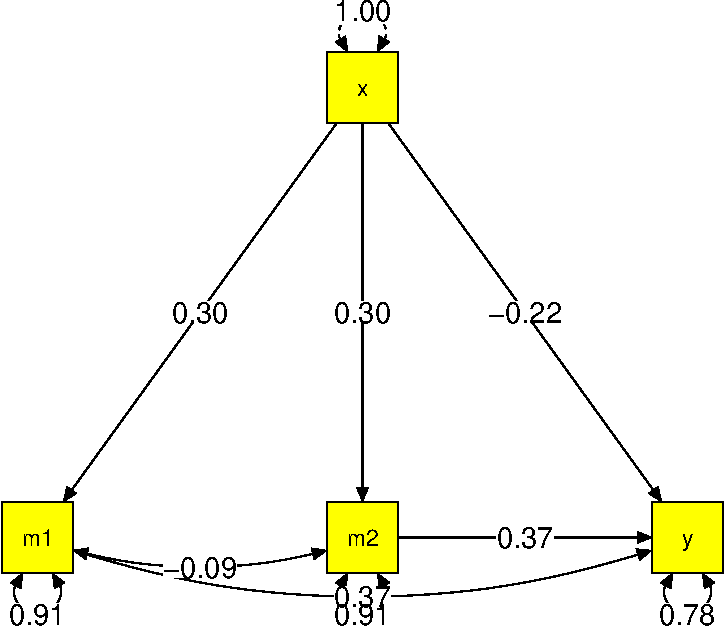
\includegraphics{Supplemental_materials_3_files/figure-latex/unnamed-chunk-2-1.pdf}

\subsection{Correct (intended to use) population correlation used to
generate the
data}\label{correct-intended-to-use-population-correlation-used-to-generate-the-data}

\begin{itemize}
\tightlist
\item
  The following \texttt{R} code shows how to derive the correct
  population correlation matrix for the model in Figure 1 in Yu et al.
\item
  We use the \texttt{impliedR()} function in the \texttt{metaSEM}
  package. Users may specify the population standardized regression
  coefficients. The function then generates the population correlation
  matrix for the model.
\item
  When we fit the model in Figure 1 to the population correlation matrix
  \texttt{CorrectP1}, the discrepancy is exact zero (\(\chi^2(df=2)=0\)
  with \(N=1,000\)). The residuals of the ``covariance'' matrix are also
  zero. The parameters are identical to the values in Figure 1 in Yu et
  al. Therefore, this is the correct population correlation matrix.
\end{itemize}

\begin{Shaded}
\begin{Highlighting}[]
\KeywordTok{library}\NormalTok{(metaSEM)}

\NormalTok{## A matrix for the regression paths as defined in Figure 1}
\NormalTok{## All of them are fixed values.}
\NormalTok{A2 <-}\StringTok{ }\KeywordTok{matrix}\NormalTok{(}\KeywordTok{c}\NormalTok{(}\DecValTok{0}\NormalTok{,}\DecValTok{0}\NormalTok{,}\DecValTok{0}\NormalTok{,}\DecValTok{0}\NormalTok{,}
               \FloatTok{0.3}\NormalTok{,}\DecValTok{0}\NormalTok{,}\DecValTok{0}\NormalTok{,}\DecValTok{0}\NormalTok{,}
               \FloatTok{0.3}\NormalTok{,}\DecValTok{0}\NormalTok{,}\DecValTok{0}\NormalTok{,}\DecValTok{0}\NormalTok{,}
               \DecValTok{0}\NormalTok{,}\FloatTok{0.3}\NormalTok{,}\FloatTok{0.3}\NormalTok{,}\DecValTok{0}\NormalTok{), }\DataTypeTok{ncol=}\DecValTok{4}\NormalTok{, }\DataTypeTok{nrow=}\DecValTok{4}\NormalTok{, }\DataTypeTok{byrow=}\OtherTok{TRUE}\NormalTok{,}
             \DataTypeTok{dimnames=}\KeywordTok{list}\NormalTok{(labels, labels))}
\NormalTok{A2}
\end{Highlighting}
\end{Shaded}

\begin{verbatim}
##      x  m1  m2 y
## x  0.0 0.0 0.0 0
## m1 0.3 0.0 0.0 0
## m2 0.3 0.0 0.0 0
## y  0.0 0.3 0.3 0
\end{verbatim}

\begin{Shaded}
\begin{Highlighting}[]
\NormalTok{## The variance of x is fixed at 1 whereas the others are starting values.}
\NormalTok{S2 <-}\StringTok{ }\KeywordTok{Diag}\NormalTok{(}\KeywordTok{c}\NormalTok{(}\DecValTok{1}\NormalTok{, }\StringTok{"0.1*Err_m1"}\NormalTok{, }\StringTok{"0.1*Err_m2"}\NormalTok{, }\StringTok{"0.1*Err_y"}\NormalTok{))}
\KeywordTok{dimnames}\NormalTok{(S2) <-}\StringTok{ }\KeywordTok{list}\NormalTok{(labels, labels)}
\NormalTok{S2}
\end{Highlighting}
\end{Shaded}

\begin{verbatim}
##    x   m1           m2           y          
## x  "1" "0"          "0"          "0"        
## m1 "0" "0.1*Err_m1" "0"          "0"        
## m2 "0" "0"          "0.1*Err_m2" "0"        
## y  "0" "0"          "0"          "0.1*Err_y"
\end{verbatim}

\begin{Shaded}
\begin{Highlighting}[]
\NormalTok{CorrectP1 <-}\StringTok{ }\KeywordTok{impliedR}\NormalTok{(A2, S2, }\DataTypeTok{labels=}\NormalTok{labels)}\OperatorTok{$}\NormalTok{SigmaObs}
\KeywordTok{kable}\NormalTok{(CorrectP1)}
\end{Highlighting}
\end{Shaded}

\begin{longtable}[]{@{}lrrrr@{}}
\toprule
& x & m1 & m2 & y\tabularnewline
\midrule
\endhead
x & 1.00 & 0.300 & 0.300 & 0.180\tabularnewline
m1 & 0.30 & 1.000 & 0.090 & 0.327\tabularnewline
m2 & 0.30 & 0.090 & 1.000 & 0.327\tabularnewline
y & 0.18 & 0.327 & 0.327 & 1.000\tabularnewline
\bottomrule
\end{longtable}

\begin{Shaded}
\begin{Highlighting}[]
\NormalTok{fit.correct1 <-}\StringTok{ }\KeywordTok{sem}\NormalTok{(model1, }\DataTypeTok{sample.cov=}\NormalTok{CorrectP1, }\DataTypeTok{sample.nobs=}\DecValTok{1000}\NormalTok{)}
\KeywordTok{summary}\NormalTok{(fit.correct1)}
\end{Highlighting}
\end{Shaded}

\begin{verbatim}
## lavaan (0.6-1) converged normally after  10 iterations
## 
##   Number of observations                          1000
## 
##   Estimator                                         ML
##   Model Fit Test Statistic                       0.000
##   Degrees of freedom                                 2
##   P-value (Chi-square)                           1.000
## 
## Parameter Estimates:
## 
##   Information                                 Expected
##   Information saturated (h1) model          Structured
##   Standard Errors                             Standard
## 
## Regressions:
##                    Estimate  Std.Err  z-value  P(>|z|)
##   m1 ~                                                
##     x                 0.300    0.030    9.945    0.000
##   m2 ~                                                
##     x                 0.300    0.030    9.945    0.000
##   y ~                                                 
##     m1                0.300    0.028   10.539    0.000
##     m2                0.300    0.028   10.539    0.000
## 
## Variances:
##                    Estimate  Std.Err  z-value  P(>|z|)
##    .m1                0.909    0.041   22.361    0.000
##    .m2                0.909    0.041   22.361    0.000
##    .y                 0.803    0.036   22.361    0.000
\end{verbatim}

\begin{Shaded}
\begin{Highlighting}[]
\NormalTok{## Residuals of the "covariance" matrix}
\KeywordTok{resid}\NormalTok{(fit.correct1)}
\end{Highlighting}
\end{Shaded}

\begin{verbatim}
## $type
## [1] "raw"
## 
## $cov
##    m1 m2 y x
## m1 0        
## m2 0  0     
## y  0  0  0  
## x  0  0  0 0
## 
## $mean
## m1 m2  y  x 
##  0  0  0  0
\end{verbatim}

\begin{Shaded}
\begin{Highlighting}[]
\KeywordTok{semPaths}\NormalTok{(fit.correct1, }\DataTypeTok{what=}\StringTok{"est"}\NormalTok{, }\DataTypeTok{edge.label.cex=}\FloatTok{1.5}\NormalTok{, }
         \DataTypeTok{sizeMan=}\DecValTok{8}\NormalTok{, }\DataTypeTok{color=}\StringTok{"lightseagreen"}\NormalTok{, }\DataTypeTok{edge.color =} \StringTok{"black"}\NormalTok{, }
         \DataTypeTok{weighted=}\OtherTok{FALSE}\NormalTok{, }\DataTypeTok{layout=}\StringTok{"tree2"}\NormalTok{)}
\end{Highlighting}
\end{Shaded}

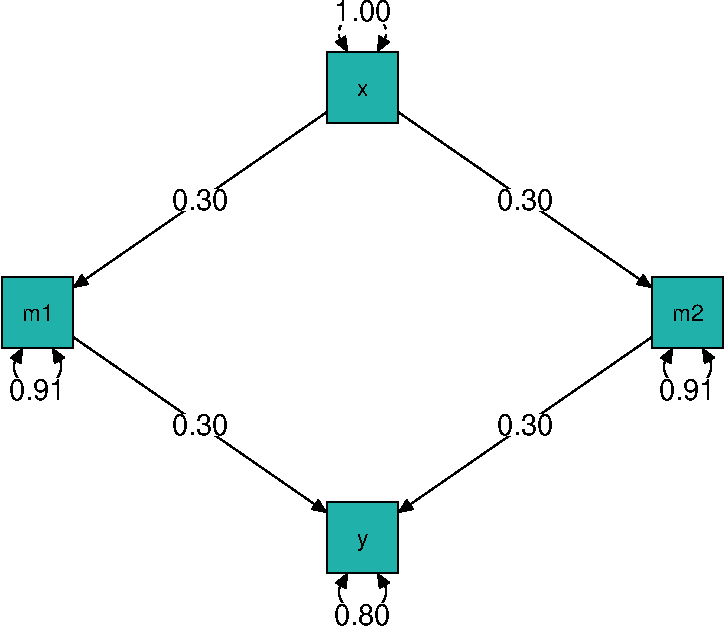
\includegraphics{Supplemental_materials_3_files/figure-latex/unnamed-chunk-4-1.pdf}

\subsection{Incorrect (actually used) model specification in analyzing
the
data}\label{incorrect-actually-used-model-specification-in-analyzing-the-data}

\begin{itemize}
\tightlist
\item
  The roles of independent and dependent variables in the \texttt{A}
  matrix in \texttt{OpenMx} and \texttt{metaSEM} were incorrectly
  reversed in Yu et al. Moreover, the error variances were incorrectly
  fixed at 1.0 in the \texttt{S} matrix. Therefore, the results in
  Figure 1 were incorrect in Yu et al.
\item
  The following was the model used in the simulation study in Yu et al.
\end{itemize}

\begin{Shaded}
\begin{Highlighting}[]
\NormalTok{varnames <-}\StringTok{ }\KeywordTok{c}\NormalTok{(}\StringTok{'X'}\NormalTok{,}\StringTok{'M1'}\NormalTok{,}\StringTok{'M2'}\NormalTok{,}\StringTok{'Y'}\NormalTok{)}

\NormalTok{A <-}\StringTok{ }\KeywordTok{mxMatrix}\NormalTok{(}\StringTok{'Full'}\NormalTok{, }\DataTypeTok{ncol=}\DecValTok{4}\NormalTok{, }\DataTypeTok{nrow=}\DecValTok{4}\NormalTok{, }\DataTypeTok{byrow=}\NormalTok{T,}
              \DataTypeTok{values =} \KeywordTok{c}\NormalTok{(}\DecValTok{0}\NormalTok{,}\FloatTok{0.3}\NormalTok{,}\FloatTok{0.3}\NormalTok{,}\DecValTok{0}\NormalTok{,}
                         \DecValTok{0}\NormalTok{,}\DecValTok{0}\NormalTok{,}\DecValTok{0}\NormalTok{,}\FloatTok{0.3}\NormalTok{,}
                         \DecValTok{0}\NormalTok{,}\DecValTok{0}\NormalTok{,}\DecValTok{0}\NormalTok{,}\FloatTok{0.3}\NormalTok{,}
                         \DecValTok{0}\NormalTok{,}\DecValTok{0}\NormalTok{,}\DecValTok{0}\NormalTok{,}\DecValTok{0}\NormalTok{),}
              \DataTypeTok{free=}\KeywordTok{c}\NormalTok{(F,T,T,F,}
\NormalTok{                     F,F,F,T,}
\NormalTok{                     F,F,F,T,}
\NormalTok{                     F,F,F,F}
\NormalTok{              ),}
              \DataTypeTok{labels=}\KeywordTok{c}\NormalTok{(}\OtherTok{NA}\NormalTok{,}\StringTok{"betaxm1"}\NormalTok{,}\StringTok{"betaxm2"}\NormalTok{,}\OtherTok{NA}\NormalTok{,}
                       \OtherTok{NA}\NormalTok{,}\OtherTok{NA}\NormalTok{,}\OtherTok{NA}\NormalTok{,}\StringTok{"betam1y"}\NormalTok{,}
                       \OtherTok{NA}\NormalTok{,}\OtherTok{NA}\NormalTok{,}\OtherTok{NA}\NormalTok{,}\StringTok{"betam2y"}\NormalTok{,}
                       \OtherTok{NA}\NormalTok{,}\OtherTok{NA}\NormalTok{,}\OtherTok{NA}\NormalTok{,}\OtherTok{NA}
\NormalTok{              ),}
              \DataTypeTok{name=}\StringTok{"A"}\NormalTok{)}

\NormalTok{S <-}\StringTok{ }\KeywordTok{mxMatrix}\NormalTok{(}\StringTok{'Full'}\NormalTok{, }\DataTypeTok{ncol=}\DecValTok{4}\NormalTok{, }\DataTypeTok{nrow=}\DecValTok{4}\NormalTok{, }\DataTypeTok{byrow=}\NormalTok{T,}
              \DataTypeTok{values =} \KeywordTok{c}\NormalTok{(}\DecValTok{1}\NormalTok{,}\DecValTok{0}\NormalTok{,}\DecValTok{0}\NormalTok{,}\DecValTok{0}\NormalTok{,}
                         \DecValTok{0}\NormalTok{,}\DecValTok{1}\NormalTok{,.}\DecValTok{2}\NormalTok{,}\DecValTok{0}\NormalTok{,}
                         \DecValTok{0}\NormalTok{,.}\DecValTok{2}\NormalTok{,}\DecValTok{1}\NormalTok{,}\DecValTok{0}\NormalTok{,}
                         \DecValTok{0}\NormalTok{,}\DecValTok{0}\NormalTok{,}\DecValTok{0}\NormalTok{,}\DecValTok{1}\NormalTok{),}
              \DataTypeTok{free=}\KeywordTok{c}\NormalTok{(F,F,F,F,}
\NormalTok{                     F,F,T,F,}
\NormalTok{                     F,T,F,F,}
\NormalTok{                     F,F,F,F),}
              \DataTypeTok{labels=}\KeywordTok{c}\NormalTok{(}\StringTok{"varx"}\NormalTok{,}\OtherTok{NA}\NormalTok{,}\OtherTok{NA}\NormalTok{,}\OtherTok{NA}\NormalTok{,}
                       \OtherTok{NA}\NormalTok{,}\StringTok{"varm1"}\NormalTok{,}\StringTok{"covm1m2"}\NormalTok{,}\OtherTok{NA}\NormalTok{,}
                       \OtherTok{NA}\NormalTok{,}\StringTok{"covm1m2"}\NormalTok{,}\StringTok{"varm2"}\NormalTok{,}\OtherTok{NA}\NormalTok{,}
                       \OtherTok{NA}\NormalTok{,}\OtherTok{NA}\NormalTok{,}\OtherTok{NA}\NormalTok{,}\StringTok{"vary"}
\NormalTok{              ),}
              \DataTypeTok{name=}\StringTok{"S"}\NormalTok{)}

\NormalTok{## Extract the values and draw the model}
\NormalTok{Amatrix <-}\StringTok{ }\NormalTok{A}\OperatorTok{$}\NormalTok{values}
\KeywordTok{dimnames}\NormalTok{(Amatrix) <-}\StringTok{ }\KeywordTok{list}\NormalTok{(labels, labels)}
\NormalTok{Amatrix}
\end{Highlighting}
\end{Shaded}

\begin{verbatim}
##    x  m1  m2   y
## x  0 0.3 0.3 0.0
## m1 0 0.0 0.0 0.3
## m2 0 0.0 0.0 0.3
## y  0 0.0 0.0 0.0
\end{verbatim}

\begin{Shaded}
\begin{Highlighting}[]
\NormalTok{Smatrix <-}\StringTok{ }\NormalTok{S}\OperatorTok{$}\NormalTok{values}
\KeywordTok{dimnames}\NormalTok{(Smatrix) <-}\StringTok{ }\KeywordTok{list}\NormalTok{(labels, labels)}
\NormalTok{Smatrix}
\end{Highlighting}
\end{Shaded}

\begin{verbatim}
##    x  m1  m2 y
## x  1 0.0 0.0 0
## m1 0 1.0 0.2 0
## m2 0 0.2 1.0 0
## y  0 0.0 0.0 1
\end{verbatim}

\begin{Shaded}
\begin{Highlighting}[]
\NormalTok{Fmatrix <-}\StringTok{ }\KeywordTok{diag}\NormalTok{(}\DecValTok{4}\NormalTok{)}

\NormalTok{incorrect.plot <-}\StringTok{ }\KeywordTok{ramModel}\NormalTok{(Amatrix, Smatrix, Fmatrix, }\DataTypeTok{manNames=}\NormalTok{varnames)}

\NormalTok{## All the directions are incorrect.}
\KeywordTok{semPaths}\NormalTok{(incorrect.plot, }\DataTypeTok{layout=}\StringTok{"tree2"}\NormalTok{, }\DataTypeTok{sizeMan=}\DecValTok{8}\NormalTok{, }\DataTypeTok{edge.color =} \StringTok{"black"}\NormalTok{, }
         \DataTypeTok{whatLabels =} \StringTok{"hide"}\NormalTok{, }\DataTypeTok{color=}\StringTok{"yellow"}\NormalTok{)}
\end{Highlighting}
\end{Shaded}

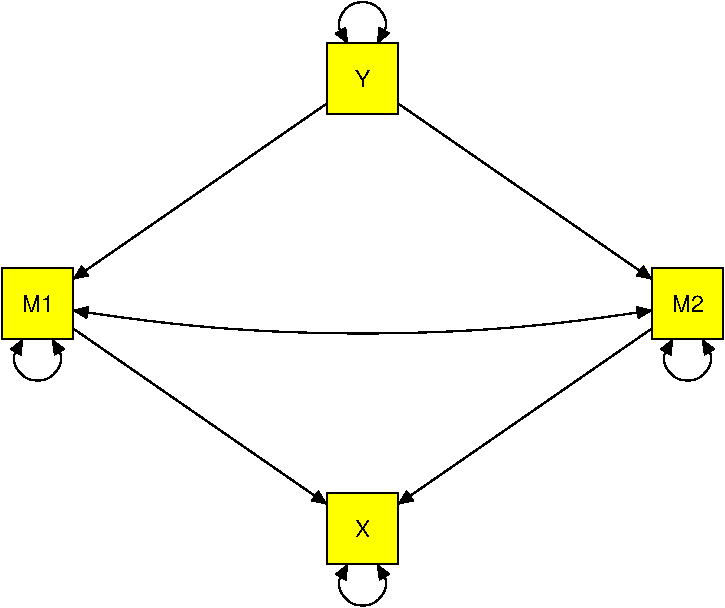
\includegraphics{Supplemental_materials_3_files/figure-latex/unnamed-chunk-6-1.pdf}

\subsection{Correct (intended to use) model specification in analyzing
the
data}\label{correct-intended-to-use-model-specification-in-analyzing-the-data}

\begin{itemize}
\tightlist
\item
  The following is the correct model specified in Figure 1 in Yu et al.
\item
  There is no correlation between the residuals in the generating model.
  We include it to follow the model specified in Yu et al.
\end{itemize}

\begin{Shaded}
\begin{Highlighting}[]
\NormalTok{A <-}\StringTok{ }\KeywordTok{create.mxMatrix}\NormalTok{(}\KeywordTok{c}\NormalTok{(}\DecValTok{0}\NormalTok{,}\DecValTok{0}\NormalTok{,}\DecValTok{0}\NormalTok{,}\DecValTok{0}\NormalTok{,}
                       \StringTok{"0.3*betaxm1"}\NormalTok{,}\DecValTok{0}\NormalTok{,}\DecValTok{0}\NormalTok{,}\DecValTok{0}\NormalTok{,}
                       \StringTok{"0.3*betaxm2"}\NormalTok{,}\DecValTok{0}\NormalTok{,}\DecValTok{0}\NormalTok{,}\DecValTok{0}\NormalTok{,}
                       \DecValTok{0}\NormalTok{,}\StringTok{"0.3*betam1y"}\NormalTok{,}\StringTok{"0.3*betam2y"}\NormalTok{,}\DecValTok{0}\NormalTok{), }
                     \DataTypeTok{ncol=}\DecValTok{4}\NormalTok{, }\DataTypeTok{nrow=}\DecValTok{4}\NormalTok{, }\DataTypeTok{byrow=}\OtherTok{TRUE}\NormalTok{, }\DataTypeTok{name=}\StringTok{"A"}\NormalTok{)}

\NormalTok{S <-}\StringTok{ }\KeywordTok{create.mxMatrix}\NormalTok{(}\KeywordTok{c}\NormalTok{(}\DecValTok{1}\NormalTok{,}
                       \DecValTok{0}\NormalTok{,}\StringTok{"0.2*varm1"}\NormalTok{,}
                       \DecValTok{0}\NormalTok{,}\StringTok{"0.1*covm1m2"}\NormalTok{,}\StringTok{"0.2*varm2"}\NormalTok{,}
                       \DecValTok{0}\NormalTok{,}\DecValTok{0}\NormalTok{,}\DecValTok{0}\NormalTok{,}\StringTok{"0.2*vary"}\NormalTok{), }
                     \DataTypeTok{type=}\StringTok{"Symm"}\NormalTok{, }\DataTypeTok{ncol=}\DecValTok{4}\NormalTok{, }\DataTypeTok{nrow=}\DecValTok{4}\NormalTok{, }\DataTypeTok{byrow=}\OtherTok{TRUE}\NormalTok{, }\DataTypeTok{name=}\StringTok{"S"}\NormalTok{)}

\NormalTok{## Extract the values and draw the model}
\NormalTok{Amatrix <-}\StringTok{ }\NormalTok{A}\OperatorTok{$}\NormalTok{values}
\KeywordTok{dimnames}\NormalTok{(Amatrix) <-}\StringTok{ }\KeywordTok{list}\NormalTok{(labels, labels)}
\NormalTok{Amatrix}
\end{Highlighting}
\end{Shaded}

\begin{verbatim}
##      x  m1  m2 y
## x  0.0 0.0 0.0 0
## m1 0.3 0.0 0.0 0
## m2 0.3 0.0 0.0 0
## y  0.0 0.3 0.3 0
\end{verbatim}

\begin{Shaded}
\begin{Highlighting}[]
\NormalTok{Smatrix <-}\StringTok{ }\NormalTok{S}\OperatorTok{$}\NormalTok{values}
\KeywordTok{dimnames}\NormalTok{(Smatrix) <-}\StringTok{ }\KeywordTok{list}\NormalTok{(labels, labels)}
\NormalTok{Smatrix}
\end{Highlighting}
\end{Shaded}

\begin{verbatim}
##    x  m1  m2   y
## x  1 0.0 0.0 0.0
## m1 0 0.2 0.1 0.0
## m2 0 0.1 0.2 0.0
## y  0 0.0 0.0 0.2
\end{verbatim}

\begin{Shaded}
\begin{Highlighting}[]
\NormalTok{correct.plot <-}\StringTok{ }\KeywordTok{ramModel}\NormalTok{(Amatrix, Smatrix, Fmatrix, }\DataTypeTok{manNames=}\NormalTok{varnames)}

\NormalTok{## All the directions are correct.}
\KeywordTok{semPaths}\NormalTok{(correct.plot, }\DataTypeTok{layout=}\StringTok{"tree2"}\NormalTok{, }\DataTypeTok{sizeMan=}\DecValTok{8}\NormalTok{, }\DataTypeTok{edge.color =} \StringTok{"black"}\NormalTok{, }
         \DataTypeTok{whatLabels =} \StringTok{"hide"}\NormalTok{, }\DataTypeTok{color=}\StringTok{"lightseagreen"}\NormalTok{)}
\end{Highlighting}
\end{Shaded}

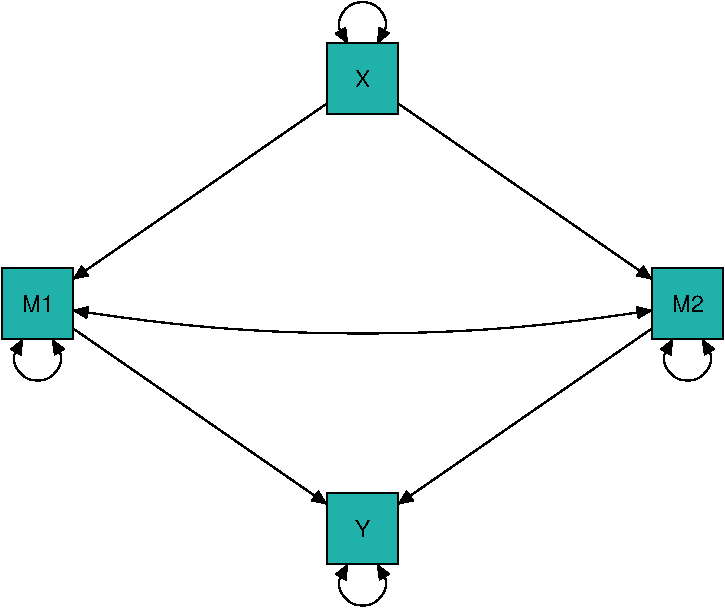
\includegraphics{Supplemental_materials_3_files/figure-latex/unnamed-chunk-7-1.pdf}

\section{Figure 2 in Yu et al. (2016)}\label{figure-2-in-yu-et-al.-2016}

\subsection{Incorrect (actually used) population correlation used to
generate the
data}\label{incorrect-actually-used-population-correlation-used-to-generate-the-data-1}

\begin{itemize}
\tightlist
\item
  The same errors were also observed in Figure 2 in Yu et al. Pearson
  correlations were incorrectly used to represent the path coefficients
  to generate the random correlation matrices.
\item
  The incorrect population correlation matrix \texttt{IncorrectP2} was
  used to generate data in Run 6 Study 1 and their online
  Supplemental-Material-2.docx.
\item
  If we use \texttt{IncorrectP2} (the population values) to fit the
  proposed path model in Figure 2, the value of the discrepancy function
  is non-zero (\(\chi^2(df=8)=1,276.262\) with \(N=1,000\)). Moreover,
  the residuals of the ``covariance'' matrix are non-zero. This shows
  that the population correlation matrix \texttt{IncorrectP2} does not
  match the model in Figure 2.
\end{itemize}

\begin{Shaded}
\begin{Highlighting}[]
\NormalTok{labels <-}\StringTok{ }\KeywordTok{c}\NormalTok{(}\StringTok{"x1"}\NormalTok{,}\StringTok{"x2"}\NormalTok{,}\StringTok{"x3"}\NormalTok{,}\StringTok{"m1"}\NormalTok{,}\StringTok{"m2"}\NormalTok{,}\StringTok{"y1"}\NormalTok{,}\StringTok{"y2"}\NormalTok{)}

\NormalTok{## These are the values used as the population correlation matrix }
\NormalTok{## to generate the data in Figure 2}
\NormalTok{rho <-}\StringTok{ }\FloatTok{0.3}
\NormalTok{r <-}\StringTok{ }\KeywordTok{c}\NormalTok{(}\DecValTok{0}\NormalTok{,}\DecValTok{0}\NormalTok{,rho,rho,}\DecValTok{0}\NormalTok{,}\DecValTok{0}\NormalTok{,}\DecValTok{0}\NormalTok{,rho,rho,}\DecValTok{0}\NormalTok{,}\DecValTok{0}\NormalTok{,rho,rho,}\DecValTok{0}\NormalTok{,}\DecValTok{0}\NormalTok{,}\DecValTok{0}\NormalTok{,rho,rho,rho,rho,}\DecValTok{0}\NormalTok{)}
\NormalTok{IncorrectP2 <-}\StringTok{ }\KeywordTok{lav_matrix_vech_reverse}\NormalTok{(r, }\DataTypeTok{diagonal=}\OtherTok{FALSE}\NormalTok{)}
\KeywordTok{diag}\NormalTok{(IncorrectP2) <-}\StringTok{ }\DecValTok{1}
\KeywordTok{dimnames}\NormalTok{(IncorrectP2) <-}\StringTok{ }\KeywordTok{list}\NormalTok{(labels, labels)}

\KeywordTok{kable}\NormalTok{(IncorrectP2)}
\end{Highlighting}
\end{Shaded}

\begin{longtable}[]{@{}lrrrrrrr@{}}
\toprule
& x1 & x2 & x3 & m1 & m2 & y1 & y2\tabularnewline
\midrule
\endhead
x1 & 1.0 & 0.0 & 0.0 & 0.3 & 0.3 & 0.0 & 0.0\tabularnewline
x2 & 0.0 & 1.0 & 0.0 & 0.3 & 0.3 & 0.0 & 0.0\tabularnewline
x3 & 0.0 & 0.0 & 1.0 & 0.3 & 0.3 & 0.0 & 0.0\tabularnewline
m1 & 0.3 & 0.3 & 0.3 & 1.0 & 0.0 & 0.3 & 0.3\tabularnewline
m2 & 0.3 & 0.3 & 0.3 & 0.0 & 1.0 & 0.3 & 0.3\tabularnewline
y1 & 0.0 & 0.0 & 0.0 & 0.3 & 0.3 & 1.0 & 0.0\tabularnewline
y2 & 0.0 & 0.0 & 0.0 & 0.3 & 0.3 & 0.0 & 1.0\tabularnewline
\bottomrule
\end{longtable}

\begin{Shaded}
\begin{Highlighting}[]
\NormalTok{## Population model: no direct effect used in the analysis}
\NormalTok{model3 <-}\StringTok{ 'm1 + m2 ~ x1 + x2 + x3}
\StringTok{           y1 + y2 ~ m1 + m2}
\StringTok{           y1 ~~ 0*y2'}

\NormalTok{## Incorrect model. The fit is not perfect even the population correlation matrix is used.}
\NormalTok{fit.incorrect3 <-}\StringTok{ }\KeywordTok{sem}\NormalTok{(model3, }\DataTypeTok{sample.cov=}\NormalTok{IncorrectP2, }\DataTypeTok{sample.nobs=}\DecValTok{1000}\NormalTok{)}
\KeywordTok{summary}\NormalTok{(fit.incorrect3)  }
\end{Highlighting}
\end{Shaded}

\begin{verbatim}
## lavaan (0.6-1) converged normally after   9 iterations
## 
##   Number of observations                          1000
## 
##   Estimator                                         ML
##   Model Fit Test Statistic                    1276.262
##   Degrees of freedom                                 8
##   P-value (Chi-square)                           0.000
## 
## Parameter Estimates:
## 
##   Information                                 Expected
##   Information saturated (h1) model          Structured
##   Standard Errors                             Standard
## 
## Regressions:
##                    Estimate  Std.Err  z-value  P(>|z|)
##   m1 ~                                                
##     x1                0.300    0.027   11.103    0.000
##     x2                0.300    0.027   11.103    0.000
##     x3                0.300    0.027   11.103    0.000
##   m2 ~                                                
##     x1                0.300    0.027   11.103    0.000
##     x2                0.300    0.027   11.103    0.000
##     x3                0.300    0.027   11.103    0.000
##   y1 ~                                                
##     m1                0.300    0.030   10.087    0.000
##     m2                0.300    0.030   10.087    0.000
##   y2 ~                                                
##     m1                0.300    0.030   10.087    0.000
##     m2                0.300    0.030   10.087    0.000
## 
## Covariances:
##                    Estimate  Std.Err  z-value  P(>|z|)
##  .y1 ~~                                               
##    .y2                0.000                           
## 
## Variances:
##                    Estimate  Std.Err  z-value  P(>|z|)
##    .m1                0.729    0.033   22.361    0.000
##    .m2                0.729    0.033   22.361    0.000
##    .y1                0.819    0.037   22.361    0.000
##    .y2                0.819    0.037   22.361    0.000
\end{verbatim}

\begin{Shaded}
\begin{Highlighting}[]
\NormalTok{## Residuals of the "covariance" matrix}
\KeywordTok{resid}\NormalTok{(fit.incorrect3)}
\end{Highlighting}
\end{Shaded}

\begin{verbatim}
## $type
## [1] "raw"
## 
## $cov
##    m1     m2     y1     y2     x1     x2     x3    
## m1  0.000                                          
## m2 -0.270  0.000                                   
## y1 -0.081 -0.081 -0.049                            
## y2 -0.081 -0.081 -0.228 -0.049                     
## x1  0.000  0.000 -0.180 -0.180  0.000              
## x2  0.000  0.000 -0.180 -0.180  0.000  0.000       
## x3  0.000  0.000 -0.180 -0.180  0.000  0.000  0.000
## 
## $mean
## m1 m2 y1 y2 x1 x2 x3 
##  0  0  0  0  0  0  0
\end{verbatim}

\begin{itemize}
\tightlist
\item
  To see what the actual generating model is, we add the direct effects
  and the correlated residuals. The model is now saturated. The results
  show that there are negative direct effects (-0.391) from \(x1\),
  \(x2\) and \(x3\) to \(y1\) and \(y2\). Moreover, there are correlated
  residuals between \(m1\) and \(m2\), and between \(y1\) and \(y2\).
  This model is different from the one in Figure 2 in Yu et al.
\end{itemize}

\begin{Shaded}
\begin{Highlighting}[]
\NormalTok{## Population model: no direct effect used in the analysis}
\NormalTok{model4 <-}\StringTok{ 'y1 + y2 + m1 + m2 ~ x1 + x2 + x3}
\StringTok{           y1 + y2 ~ m1 + m2 }
\StringTok{           m1 ~~ m2}
\StringTok{           y1 ~~ y2'}

\NormalTok{## Incorrect model. The fit is not perfect even population correlation matrix is used.}
\NormalTok{fit.incorrect4 <-}\StringTok{ }\KeywordTok{sem}\NormalTok{(model4, }\DataTypeTok{sample.cov=}\NormalTok{IncorrectP2, }\DataTypeTok{sample.nobs=}\DecValTok{1000}\NormalTok{)}
\KeywordTok{summary}\NormalTok{(fit.incorrect4)}
\end{Highlighting}
\end{Shaded}

\begin{verbatim}
## lavaan (0.6-1) converged normally after  19 iterations
## 
##   Number of observations                          1000
## 
##   Estimator                                         ML
##   Model Fit Test Statistic                       0.000
##   Degrees of freedom                                 0
## 
## Parameter Estimates:
## 
##   Information                                 Expected
##   Information saturated (h1) model          Structured
##   Standard Errors                             Standard
## 
## Regressions:
##                    Estimate  Std.Err  z-value  P(>|z|)
##   y1 ~                                                
##     x1               -0.391    0.029  -13.446    0.000
##     x2               -0.391    0.029  -13.446    0.000
##     x3               -0.391    0.029  -13.446    0.000
##   y2 ~                                                
##     x1               -0.391    0.029  -13.446    0.000
##     x2               -0.391    0.029  -13.446    0.000
##     x3               -0.391    0.029  -13.446    0.000
##   m1 ~                                                
##     x1                0.300    0.027   11.103    0.000
##     x2                0.300    0.027   11.103    0.000
##     x3                0.300    0.027   11.103    0.000
##   m2 ~                                                
##     x1                0.300    0.027   11.103    0.000
##     x2                0.300    0.027   11.103    0.000
##     x3                0.300    0.027   11.103    0.000
##   y1 ~                                                
##     m1                0.652    0.031   20.984    0.000
##     m2                0.652    0.031   20.984    0.000
##   y2 ~                                                
##     m1                0.652    0.031   20.984    0.000
##     m2                0.652    0.031   20.984    0.000
## 
## Covariances:
##                    Estimate  Std.Err  z-value  P(>|z|)
##  .m1 ~~                                               
##    .m2               -0.270    0.025  -10.970    0.000
##  .y1 ~~                                               
##    .y2               -0.391    0.023  -17.100    0.000
## 
## Variances:
##                    Estimate  Std.Err  z-value  P(>|z|)
##    .y1                0.608    0.027   22.361    0.000
##    .y2                0.608    0.027   22.361    0.000
##    .m1                0.729    0.033   22.361    0.000
##    .m2                0.729    0.033   22.361    0.000
\end{verbatim}

\begin{Shaded}
\begin{Highlighting}[]
\NormalTok{## Residuals of the "covariance" matrix}
\KeywordTok{resid}\NormalTok{(fit.incorrect4)}
\end{Highlighting}
\end{Shaded}

\begin{verbatim}
## $type
## [1] "raw"
## 
## $cov
##    y1 y2 m1 m2 x1 x2 x3
## y1 0                   
## y2 0  0                
## m1 0  0  0             
## m2 0  0  0  0          
## x1 0  0  0  0  0       
## x2 0  0  0  0  0  0    
## x3 0  0  0  0  0  0  0 
## 
## $mean
## y1 y2 m1 m2 x1 x2 x3 
##  0  0  0  0  0  0  0
\end{verbatim}

\begin{Shaded}
\begin{Highlighting}[]
\KeywordTok{semPaths}\NormalTok{(fit.incorrect4, }\DataTypeTok{what=}\StringTok{"est"}\NormalTok{, }\DataTypeTok{edge.label.cex=}\FloatTok{1.5}\NormalTok{, }
         \DataTypeTok{sizeMan=}\DecValTok{8}\NormalTok{, }\DataTypeTok{color=}\StringTok{"yellow"}\NormalTok{, }\DataTypeTok{edge.color =} \StringTok{"black"}\NormalTok{, }
         \DataTypeTok{weighted=}\OtherTok{FALSE}\NormalTok{, }\DataTypeTok{layout=}\StringTok{"tree2"}\NormalTok{)}
\end{Highlighting}
\end{Shaded}

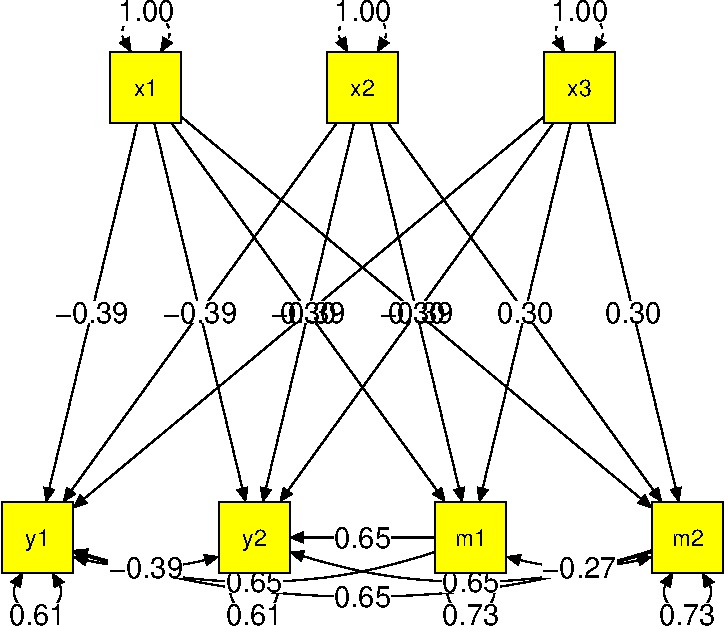
\includegraphics{Supplemental_materials_3_files/figure-latex/unnamed-chunk-9-1.pdf}

\subsection{Correct (intended to use) population correlation used to
generate the
data}\label{correct-intended-to-use-population-correlation-used-to-generate-the-data-1}

\begin{itemize}
\tightlist
\item
  The following R code shows how to generate the correct correlation
  matrix for Figure 2 in Yu et al.
\item
  We specify the regression paths in the \texttt{A4} matrix. Then we
  generate the population correlation matrix with the
  \texttt{impliedR()} function.
\item
  When we fit the model in Figure 2 to the population correlation matrix
  \texttt{CorrectP2}, the discrepancy is exact zero (\(\chi^2(df=8)=0\)
  with \(N=1,000\)). The residuals of the ``covariance'' matrix are
  zero. The parameters are identical to the values in Figure 2.
  Therefore, this is the correct population correlation matrix.
\end{itemize}

\begin{Shaded}
\begin{Highlighting}[]
\NormalTok{## A matrix for the regression paths as defined in Figure 2}
\NormalTok{## All of them are fixed values.}
\NormalTok{A4 <-}\StringTok{ }\KeywordTok{matrix}\NormalTok{(}\KeywordTok{c}\NormalTok{(}\DecValTok{0}\NormalTok{,}\DecValTok{0}\NormalTok{,}\DecValTok{0}\NormalTok{,}\DecValTok{0}\NormalTok{,}\DecValTok{0}\NormalTok{,}\DecValTok{0}\NormalTok{,}\DecValTok{0}\NormalTok{,}
               \DecValTok{0}\NormalTok{,}\DecValTok{0}\NormalTok{,}\DecValTok{0}\NormalTok{,}\DecValTok{0}\NormalTok{,}\DecValTok{0}\NormalTok{,}\DecValTok{0}\NormalTok{,}\DecValTok{0}\NormalTok{,}
               \DecValTok{0}\NormalTok{,}\DecValTok{0}\NormalTok{,}\DecValTok{0}\NormalTok{,}\DecValTok{0}\NormalTok{,}\DecValTok{0}\NormalTok{,}\DecValTok{0}\NormalTok{,}\DecValTok{0}\NormalTok{,}
               \FloatTok{0.3}\NormalTok{,}\FloatTok{0.3}\NormalTok{,}\FloatTok{0.3}\NormalTok{,}\DecValTok{0}\NormalTok{,}\DecValTok{0}\NormalTok{,}\DecValTok{0}\NormalTok{,}\DecValTok{0}\NormalTok{,}
               \FloatTok{0.3}\NormalTok{,}\FloatTok{0.3}\NormalTok{,}\FloatTok{0.3}\NormalTok{,}\DecValTok{0}\NormalTok{,}\DecValTok{0}\NormalTok{,}\DecValTok{0}\NormalTok{,}\DecValTok{0}\NormalTok{,}
               \DecValTok{0}\NormalTok{,}\DecValTok{0}\NormalTok{,}\DecValTok{0}\NormalTok{,}\FloatTok{0.3}\NormalTok{,}\FloatTok{0.3}\NormalTok{,}\DecValTok{0}\NormalTok{,}\DecValTok{0}\NormalTok{,}
               \DecValTok{0}\NormalTok{,}\DecValTok{0}\NormalTok{,}\DecValTok{0}\NormalTok{,}\FloatTok{0.3}\NormalTok{,}\FloatTok{0.3}\NormalTok{,}\DecValTok{0}\NormalTok{,}\DecValTok{0}\NormalTok{), }\DataTypeTok{ncol=}\DecValTok{7}\NormalTok{, }\DataTypeTok{nrow=}\DecValTok{7}\NormalTok{, }\DataTypeTok{byrow=}\OtherTok{TRUE}\NormalTok{,}
             \DataTypeTok{dimnames=}\KeywordTok{list}\NormalTok{(labels, labels))}
\NormalTok{A4}
\end{Highlighting}
\end{Shaded}

\begin{verbatim}
##     x1  x2  x3  m1  m2 y1 y2
## x1 0.0 0.0 0.0 0.0 0.0  0  0
## x2 0.0 0.0 0.0 0.0 0.0  0  0
## x3 0.0 0.0 0.0 0.0 0.0  0  0
## m1 0.3 0.3 0.3 0.0 0.0  0  0
## m2 0.3 0.3 0.3 0.0 0.0  0  0
## y1 0.0 0.0 0.0 0.3 0.3  0  0
## y2 0.0 0.0 0.0 0.3 0.3  0  0
\end{verbatim}

\begin{Shaded}
\begin{Highlighting}[]
\NormalTok{## The variances of x1 to x3 are fixed at 1 whereas the others are starting values.}
\NormalTok{S4 <-}\StringTok{ }\KeywordTok{Diag}\NormalTok{(}\KeywordTok{c}\NormalTok{(}\DecValTok{1}\NormalTok{,}\DecValTok{1}\NormalTok{,}\DecValTok{1}\NormalTok{,}\StringTok{"0.1*Err_m1"}\NormalTok{,}\StringTok{"0.1*Err_m2"}\NormalTok{,}\StringTok{"0.1*Err_y1"}\NormalTok{, }\StringTok{"0.1*Err_y2"}\NormalTok{))}
\KeywordTok{dimnames}\NormalTok{(S4) <-}\StringTok{ }\KeywordTok{list}\NormalTok{(labels, labels)}
\NormalTok{S4}
\end{Highlighting}
\end{Shaded}

\begin{verbatim}
##    x1  x2  x3  m1           m2           y1           y2          
## x1 "1" "0" "0" "0"          "0"          "0"          "0"         
## x2 "0" "1" "0" "0"          "0"          "0"          "0"         
## x3 "0" "0" "1" "0"          "0"          "0"          "0"         
## m1 "0" "0" "0" "0.1*Err_m1" "0"          "0"          "0"         
## m2 "0" "0" "0" "0"          "0.1*Err_m2" "0"          "0"         
## y1 "0" "0" "0" "0"          "0"          "0.1*Err_y1" "0"         
## y2 "0" "0" "0" "0"          "0"          "0"          "0.1*Err_y2"
\end{verbatim}

\begin{Shaded}
\begin{Highlighting}[]
\NormalTok{CorrectP2 <-}\StringTok{ }\KeywordTok{impliedR}\NormalTok{(A4, S4, }\DataTypeTok{labels=}\NormalTok{labels)}\OperatorTok{$}\NormalTok{SigmaObs}
\KeywordTok{kable}\NormalTok{(CorrectP2)}
\end{Highlighting}
\end{Shaded}

\begin{longtable}[]{@{}lrrrrrrr@{}}
\toprule
& x1 & x2 & x3 & m1 & m2 & y1 & y2\tabularnewline
\midrule
\endhead
x1 & 1.00 & 0.00 & 0.00 & 0.300 & 0.300 & 0.1800 & 0.1800\tabularnewline
x2 & 0.00 & 1.00 & 0.00 & 0.300 & 0.300 & 0.1800 & 0.1800\tabularnewline
x3 & 0.00 & 0.00 & 1.00 & 0.300 & 0.300 & 0.1800 & 0.1800\tabularnewline
m1 & 0.30 & 0.30 & 0.30 & 1.000 & 0.270 & 0.3810 & 0.3810\tabularnewline
m2 & 0.30 & 0.30 & 0.30 & 0.270 & 1.000 & 0.3810 & 0.3810\tabularnewline
y1 & 0.18 & 0.18 & 0.18 & 0.381 & 0.381 & 1.0000 & 0.2286\tabularnewline
y2 & 0.18 & 0.18 & 0.18 & 0.381 & 0.381 & 0.2286 & 1.0000\tabularnewline
\bottomrule
\end{longtable}

\begin{Shaded}
\begin{Highlighting}[]
\NormalTok{fit.correct2 <-}\StringTok{ }\KeywordTok{sem}\NormalTok{(model3, }\DataTypeTok{sample.cov=}\NormalTok{CorrectP2, }\DataTypeTok{sample.nobs=}\DecValTok{1000}\NormalTok{)}
\KeywordTok{summary}\NormalTok{(fit.correct2)  }
\end{Highlighting}
\end{Shaded}

\begin{verbatim}
## lavaan (0.6-1) converged normally after  10 iterations
## 
##   Number of observations                          1000
## 
##   Estimator                                         ML
##   Model Fit Test Statistic                       0.000
##   Degrees of freedom                                 8
##   P-value (Chi-square)                           1.000
## 
## Parameter Estimates:
## 
##   Information                                 Expected
##   Information saturated (h1) model          Structured
##   Standard Errors                             Standard
## 
## Regressions:
##                    Estimate  Std.Err  z-value  P(>|z|)
##   m1 ~                                                
##     x1                0.300    0.027   11.103    0.000
##     x2                0.300    0.027   11.103    0.000
##     x3                0.300    0.027   11.103    0.000
##   m2 ~                                                
##     x1                0.300    0.027   11.103    0.000
##     x2                0.300    0.027   11.103    0.000
##     x3                0.300    0.027   11.103    0.000
##   y1 ~                                                
##     m1                0.300    0.029   10.400    0.000
##     m2                0.300    0.029   10.400    0.000
##   y2 ~                                                
##     m1                0.300    0.029   10.400    0.000
##     m2                0.300    0.029   10.400    0.000
## 
## Covariances:
##                    Estimate  Std.Err  z-value  P(>|z|)
##  .y1 ~~                                               
##    .y2                0.000                           
## 
## Variances:
##                    Estimate  Std.Err  z-value  P(>|z|)
##    .m1                0.729    0.033   22.361    0.000
##    .m2                0.729    0.033   22.361    0.000
##    .y1                0.771    0.034   22.361    0.000
##    .y2                0.771    0.034   22.361    0.000
\end{verbatim}

\begin{Shaded}
\begin{Highlighting}[]
\NormalTok{## Residuals of the "covariance" matrix}
\KeywordTok{resid}\NormalTok{(fit.correct2)}
\end{Highlighting}
\end{Shaded}

\begin{verbatim}
## $type
## [1] "raw"
## 
## $cov
##    m1 m2 y1 y2 x1 x2 x3
## m1 0                   
## m2 0  0                
## y1 0  0  0             
## y2 0  0  0  0          
## x1 0  0  0  0  0       
## x2 0  0  0  0  0  0    
## x3 0  0  0  0  0  0  0 
## 
## $mean
## m1 m2 y1 y2 x1 x2 x3 
##  0  0  0  0  0  0  0
\end{verbatim}

\begin{Shaded}
\begin{Highlighting}[]
\KeywordTok{semPaths}\NormalTok{(fit.correct2, }\DataTypeTok{what=}\StringTok{"est"}\NormalTok{, }\DataTypeTok{edge.label.cex=}\FloatTok{1.5}\NormalTok{, }
         \DataTypeTok{sizeMan=}\DecValTok{8}\NormalTok{, }\DataTypeTok{color=}\StringTok{"lightseagreen"}\NormalTok{, }\DataTypeTok{edge.color =} \StringTok{"black"}\NormalTok{, }
         \DataTypeTok{weighted=}\OtherTok{FALSE}\NormalTok{, }\DataTypeTok{layout=}\StringTok{"tree2"}\NormalTok{)}
\end{Highlighting}
\end{Shaded}

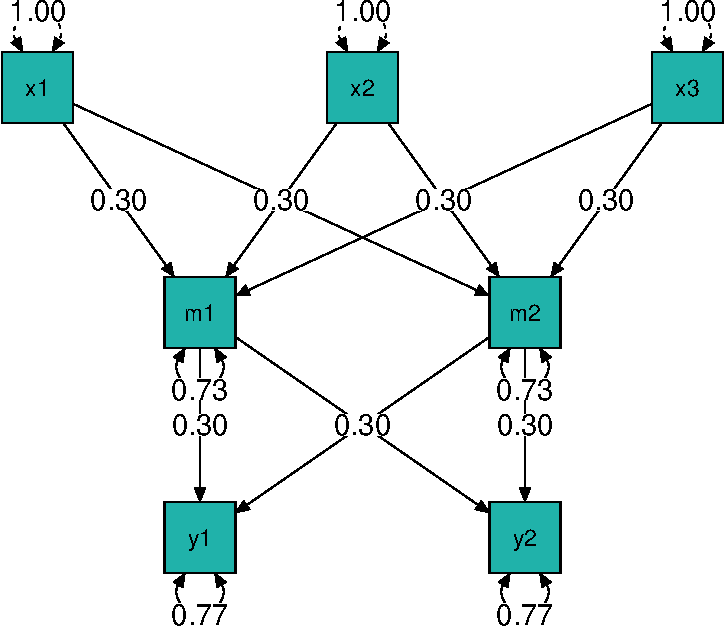
\includegraphics{Supplemental_materials_3_files/figure-latex/unnamed-chunk-11-1.pdf}

\subsection{Incorrect (actually used) model specification in analyzing
the
data}\label{incorrect-actually-used-model-specification-in-analyzing-the-data-1}

\begin{itemize}
\tightlist
\item
  The roles of independent and dependent variables in the \texttt{A}
  matrix in \texttt{OpenMx} and \texttt{metaSEM} were incorrectly
  reversed in Yu et al. Moreover, the error variances were incorrectly
  fixed at 1.0 in the \texttt{S} matrix. Therefore, the results were
  incorrect in Figure 2 in Yu et al.
\item
  The following was the model Yu et al. used in their simulation study.
\end{itemize}

\begin{Shaded}
\begin{Highlighting}[]
\NormalTok{varnames <-}\StringTok{ }\KeywordTok{c}\NormalTok{(}\StringTok{'X1'}\NormalTok{,}\StringTok{'X2'}\NormalTok{,}\StringTok{'X3'}\NormalTok{,}\StringTok{'M1'}\NormalTok{,}\StringTok{'M2'}\NormalTok{,}\StringTok{'Y1'}\NormalTok{,}\StringTok{'Y2'}\NormalTok{)}

\NormalTok{rho <-}\StringTok{ }\FloatTok{0.3}

\NormalTok{A <-}\StringTok{ }\KeywordTok{mxMatrix}\NormalTok{(}\StringTok{'Full'}\NormalTok{, }\DataTypeTok{ncol=}\DecValTok{7}\NormalTok{, }\DataTypeTok{nrow=}\DecValTok{7}\NormalTok{, }\DataTypeTok{byrow=}\NormalTok{T,}
              \DataTypeTok{values =} \KeywordTok{c}\NormalTok{(}\DecValTok{0}\NormalTok{,}\DecValTok{0}\NormalTok{,}\DecValTok{0}\NormalTok{,rho,rho,}\DecValTok{0}\NormalTok{,}\DecValTok{0}\NormalTok{,}
                         \DecValTok{0}\NormalTok{,}\DecValTok{0}\NormalTok{,}\DecValTok{0}\NormalTok{,rho,rho,}\DecValTok{0}\NormalTok{,}\DecValTok{0}\NormalTok{,}
                         \DecValTok{0}\NormalTok{,}\DecValTok{0}\NormalTok{,}\DecValTok{0}\NormalTok{,rho,rho,}\DecValTok{0}\NormalTok{,}\DecValTok{0}\NormalTok{,}
                         \DecValTok{0}\NormalTok{,}\DecValTok{0}\NormalTok{,}\DecValTok{0}\NormalTok{,}\DecValTok{0}\NormalTok{,}\DecValTok{0}\NormalTok{,rho,rho,}
                         \DecValTok{0}\NormalTok{,}\DecValTok{0}\NormalTok{,}\DecValTok{0}\NormalTok{,}\DecValTok{0}\NormalTok{,}\DecValTok{0}\NormalTok{,rho,rho,}
                         \DecValTok{0}\NormalTok{,}\DecValTok{0}\NormalTok{,}\DecValTok{0}\NormalTok{,}\DecValTok{0}\NormalTok{,}\DecValTok{0}\NormalTok{,}\DecValTok{0}\NormalTok{,}\DecValTok{0}\NormalTok{,}
                         \DecValTok{0}\NormalTok{,}\DecValTok{0}\NormalTok{,}\DecValTok{0}\NormalTok{,}\DecValTok{0}\NormalTok{,}\DecValTok{0}\NormalTok{,}\DecValTok{0}\NormalTok{,}\DecValTok{0}\NormalTok{),}
              \DataTypeTok{free=}\KeywordTok{c}\NormalTok{(F,F,F,T,T,F,F,}
\NormalTok{                     F,F,F,T,T,F,F,}
\NormalTok{                     F,F,F,T,T,F,F,}
\NormalTok{                     F,F,F,F,F,T,T,}
\NormalTok{                     F,F,F,F,F,T,T,}
\NormalTok{                     F,F,F,F,F,F,F,}
\NormalTok{                     F,F,F,F,F,F,F}
\NormalTok{              ),}
              \DataTypeTok{labels=}\KeywordTok{c}\NormalTok{(}\OtherTok{NA}\NormalTok{,}\OtherTok{NA}\NormalTok{,}\OtherTok{NA}\NormalTok{,}\StringTok{"betax1m1"}\NormalTok{,}\StringTok{"betax1m2"}\NormalTok{,}\OtherTok{NA}\NormalTok{,}\OtherTok{NA}\NormalTok{,}
                       \OtherTok{NA}\NormalTok{,}\OtherTok{NA}\NormalTok{,}\OtherTok{NA}\NormalTok{,}\StringTok{"betax2m1"}\NormalTok{,}\StringTok{"betax2m2"}\NormalTok{,}\OtherTok{NA}\NormalTok{,}\OtherTok{NA}\NormalTok{,}
                       \OtherTok{NA}\NormalTok{,}\OtherTok{NA}\NormalTok{,}\OtherTok{NA}\NormalTok{,}\StringTok{"betax3m1"}\NormalTok{,}\StringTok{"betax3m2"}\NormalTok{,}\OtherTok{NA}\NormalTok{,}\OtherTok{NA}\NormalTok{,}
                       \OtherTok{NA}\NormalTok{,}\OtherTok{NA}\NormalTok{,}\OtherTok{NA}\NormalTok{,}\OtherTok{NA}\NormalTok{,}\OtherTok{NA}\NormalTok{,}\StringTok{"betam1y1"}\NormalTok{,}\StringTok{"betam1y2"}\NormalTok{,}
                       \OtherTok{NA}\NormalTok{,}\OtherTok{NA}\NormalTok{,}\OtherTok{NA}\NormalTok{,}\OtherTok{NA}\NormalTok{,}\OtherTok{NA}\NormalTok{,}\StringTok{"betam2y1"}\NormalTok{,}\StringTok{"betam2y2"}\NormalTok{,}
                       \OtherTok{NA}\NormalTok{,}\OtherTok{NA}\NormalTok{,}\OtherTok{NA}\NormalTok{,}\OtherTok{NA}\NormalTok{,}\OtherTok{NA}\NormalTok{,}\OtherTok{NA}\NormalTok{,}\OtherTok{NA}\NormalTok{,}
                       \OtherTok{NA}\NormalTok{,}\OtherTok{NA}\NormalTok{,}\OtherTok{NA}\NormalTok{,}\OtherTok{NA}\NormalTok{,}\OtherTok{NA}\NormalTok{,}\OtherTok{NA}\NormalTok{,}\OtherTok{NA}
\NormalTok{              ),}
              \DataTypeTok{name=}\StringTok{"A"}\NormalTok{)}

\NormalTok{S <-}\StringTok{ }\KeywordTok{mxMatrix}\NormalTok{(}\StringTok{'Full'}\NormalTok{,}\DataTypeTok{ncol=}\DecValTok{7}\NormalTok{,}\DataTypeTok{nrow=}\DecValTok{7}\NormalTok{,}\DataTypeTok{byrow=}\NormalTok{T,}
              \DataTypeTok{values =} \KeywordTok{c}\NormalTok{(}\DecValTok{1}\NormalTok{,}\DecValTok{0}\NormalTok{,}\DecValTok{0}\NormalTok{,}\DecValTok{0}\NormalTok{,}\DecValTok{0}\NormalTok{,}\DecValTok{0}\NormalTok{,}\DecValTok{0}\NormalTok{,}
                         \DecValTok{0}\NormalTok{,}\DecValTok{1}\NormalTok{,}\DecValTok{0}\NormalTok{,}\DecValTok{0}\NormalTok{,}\DecValTok{0}\NormalTok{,}\DecValTok{0}\NormalTok{,}\DecValTok{0}\NormalTok{,}
                         \DecValTok{0}\NormalTok{,}\DecValTok{0}\NormalTok{,}\DecValTok{1}\NormalTok{,}\DecValTok{0}\NormalTok{,}\DecValTok{0}\NormalTok{,}\DecValTok{0}\NormalTok{,}\DecValTok{0}\NormalTok{,}
                         \DecValTok{0}\NormalTok{,}\DecValTok{0}\NormalTok{,}\DecValTok{0}\NormalTok{,}\DecValTok{1}\NormalTok{,}\FloatTok{0.1}\NormalTok{,}\DecValTok{0}\NormalTok{,}\DecValTok{0}\NormalTok{,}
                         \DecValTok{0}\NormalTok{,}\DecValTok{0}\NormalTok{,}\DecValTok{0}\NormalTok{,}\FloatTok{0.1}\NormalTok{,}\DecValTok{1}\NormalTok{,}\DecValTok{0}\NormalTok{,}\DecValTok{0}\NormalTok{,}
                         \DecValTok{0}\NormalTok{,}\DecValTok{0}\NormalTok{,}\DecValTok{0}\NormalTok{,}\DecValTok{0}\NormalTok{,}\DecValTok{0}\NormalTok{,}\DecValTok{1}\NormalTok{,}\FloatTok{0.1}\NormalTok{,}
                         \DecValTok{0}\NormalTok{,}\DecValTok{0}\NormalTok{,}\DecValTok{0}\NormalTok{,}\DecValTok{0}\NormalTok{,}\DecValTok{0}\NormalTok{,}\FloatTok{0.1}\NormalTok{,}\DecValTok{1}
\NormalTok{              ),}
              \DataTypeTok{free=}\KeywordTok{c}\NormalTok{(F,F,F,F,F,F,F,}
\NormalTok{                     F,F,F,F,F,F,F,}
\NormalTok{                     F,F,F,F,F,F,F,}
\NormalTok{                     F,F,F,F,T,F,F,}
\NormalTok{                     F,F,F,T,F,F,F,}
\NormalTok{                     F,F,F,F,F,F,T,}
\NormalTok{                     F,F,F,F,F,T,F}
\NormalTok{              ),}
              \DataTypeTok{labels=}\KeywordTok{c}\NormalTok{(}\StringTok{"varx1"}\NormalTok{,}\OtherTok{NA}\NormalTok{,}\OtherTok{NA}\NormalTok{,}\OtherTok{NA}\NormalTok{,}\OtherTok{NA}\NormalTok{,}\OtherTok{NA}\NormalTok{,}\OtherTok{NA}\NormalTok{,}
                       \OtherTok{NA}\NormalTok{,}\StringTok{"varx2"}\NormalTok{,}\OtherTok{NA}\NormalTok{,}\OtherTok{NA}\NormalTok{,}\OtherTok{NA}\NormalTok{,}\OtherTok{NA}\NormalTok{,}\OtherTok{NA}\NormalTok{,}
                       \OtherTok{NA}\NormalTok{,}\OtherTok{NA}\NormalTok{,}\StringTok{"varx3"}\NormalTok{,}\OtherTok{NA}\NormalTok{,}\OtherTok{NA}\NormalTok{,}\OtherTok{NA}\NormalTok{,}\OtherTok{NA}\NormalTok{,}
                       \OtherTok{NA}\NormalTok{,}\OtherTok{NA}\NormalTok{,}\OtherTok{NA}\NormalTok{,}\StringTok{"varm1"}\NormalTok{,}\StringTok{"covm1m2"}\NormalTok{,}\OtherTok{NA}\NormalTok{,}\OtherTok{NA}\NormalTok{,}
                       \OtherTok{NA}\NormalTok{,}\OtherTok{NA}\NormalTok{,}\OtherTok{NA}\NormalTok{,}\StringTok{"covm1m2"}\NormalTok{,}\StringTok{"varm2"}\NormalTok{,}\OtherTok{NA}\NormalTok{,}\OtherTok{NA}\NormalTok{,}
                       \OtherTok{NA}\NormalTok{,}\OtherTok{NA}\NormalTok{,}\OtherTok{NA}\NormalTok{,}\OtherTok{NA}\NormalTok{,}\OtherTok{NA}\NormalTok{,}\StringTok{"vary1"}\NormalTok{,}\StringTok{"covy1y2"}\NormalTok{,}
                       \OtherTok{NA}\NormalTok{,}\OtherTok{NA}\NormalTok{,}\OtherTok{NA}\NormalTok{,}\OtherTok{NA}\NormalTok{,}\OtherTok{NA}\NormalTok{,}\StringTok{"covy1y2"}\NormalTok{,}\StringTok{"vary2"}
\NormalTok{              ),}
              \DataTypeTok{name=}\StringTok{"S"}\NormalTok{)}

\NormalTok{## Extract the values and draw the model}
\NormalTok{Amatrix <-}\StringTok{ }\NormalTok{A}\OperatorTok{$}\NormalTok{values}
\KeywordTok{dimnames}\NormalTok{(Amatrix) <-}\StringTok{ }\KeywordTok{list}\NormalTok{(labels, labels)}
\NormalTok{Amatrix}
\end{Highlighting}
\end{Shaded}

\begin{verbatim}
##    x1 x2 x3  m1  m2  y1  y2
## x1  0  0  0 0.3 0.3 0.0 0.0
## x2  0  0  0 0.3 0.3 0.0 0.0
## x3  0  0  0 0.3 0.3 0.0 0.0
## m1  0  0  0 0.0 0.0 0.3 0.3
## m2  0  0  0 0.0 0.0 0.3 0.3
## y1  0  0  0 0.0 0.0 0.0 0.0
## y2  0  0  0 0.0 0.0 0.0 0.0
\end{verbatim}

\begin{Shaded}
\begin{Highlighting}[]
\NormalTok{Smatrix <-}\StringTok{ }\NormalTok{S}\OperatorTok{$}\NormalTok{values}
\KeywordTok{dimnames}\NormalTok{(Smatrix) <-}\StringTok{ }\KeywordTok{list}\NormalTok{(labels, labels)}
\NormalTok{Smatrix}
\end{Highlighting}
\end{Shaded}

\begin{verbatim}
##    x1 x2 x3  m1  m2  y1  y2
## x1  1  0  0 0.0 0.0 0.0 0.0
## x2  0  1  0 0.0 0.0 0.0 0.0
## x3  0  0  1 0.0 0.0 0.0 0.0
## m1  0  0  0 1.0 0.1 0.0 0.0
## m2  0  0  0 0.1 1.0 0.0 0.0
## y1  0  0  0 0.0 0.0 1.0 0.1
## y2  0  0  0 0.0 0.0 0.1 1.0
\end{verbatim}

\begin{Shaded}
\begin{Highlighting}[]
\NormalTok{Fmatrix <-}\StringTok{ }\KeywordTok{diag}\NormalTok{(}\DecValTok{7}\NormalTok{)}

\NormalTok{incorrect.plot <-}\StringTok{ }\KeywordTok{ramModel}\NormalTok{(Amatrix, Smatrix, Fmatrix, }\DataTypeTok{manNames=}\NormalTok{varnames)}

\NormalTok{## All the directions are incorrect.}
\KeywordTok{semPaths}\NormalTok{(incorrect.plot, }\DataTypeTok{layout=}\StringTok{"tree2"}\NormalTok{, }\DataTypeTok{sizeMan=}\DecValTok{8}\NormalTok{, }\DataTypeTok{edge.color =} \StringTok{"black"}\NormalTok{, }
         \DataTypeTok{whatLabels =} \StringTok{"hide"}\NormalTok{, }\DataTypeTok{color=}\StringTok{"yellow"}\NormalTok{)}
\end{Highlighting}
\end{Shaded}

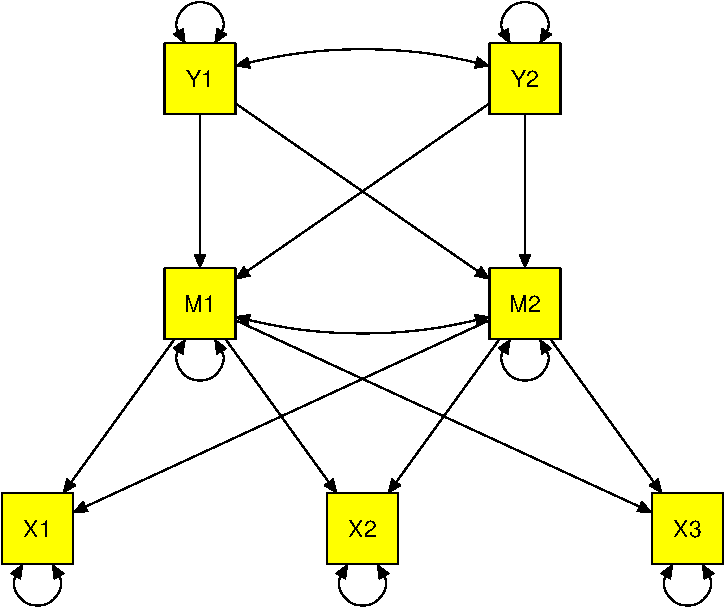
\includegraphics{Supplemental_materials_3_files/figure-latex/unnamed-chunk-13-1.pdf}

\subsection{Correct (intended to use) model specification in analyzing
the
data}\label{correct-intended-to-use-model-specification-in-analyzing-the-data-1}

\begin{itemize}
\tightlist
\item
  The following is the correct model for Figure 2 in Yu et al.
\item
  There is no correlation between the residuals in the generating model.
  We include them to follow the model specified in Yu et al.
\end{itemize}

\begin{Shaded}
\begin{Highlighting}[]
\NormalTok{varnames <-}\StringTok{ }\KeywordTok{c}\NormalTok{(}\StringTok{'X1'}\NormalTok{,}\StringTok{'X2'}\NormalTok{,}\StringTok{'X3'}\NormalTok{,}\StringTok{'M1'}\NormalTok{,}\StringTok{'M2'}\NormalTok{,}\StringTok{'Y1'}\NormalTok{,}\StringTok{'Y2'}\NormalTok{)}

\NormalTok{A <-}\StringTok{ }\KeywordTok{create.mxMatrix}\NormalTok{(}\KeywordTok{c}\NormalTok{(}\DecValTok{0}\NormalTok{,}\DecValTok{0}\NormalTok{,}\DecValTok{0}\NormalTok{,}\DecValTok{0}\NormalTok{,}\DecValTok{0}\NormalTok{,}\DecValTok{0}\NormalTok{,}\DecValTok{0}\NormalTok{,}
                       \DecValTok{0}\NormalTok{,}\DecValTok{0}\NormalTok{,}\DecValTok{0}\NormalTok{,}\DecValTok{0}\NormalTok{,}\DecValTok{0}\NormalTok{,}\DecValTok{0}\NormalTok{,}\DecValTok{0}\NormalTok{,}
                       \DecValTok{0}\NormalTok{,}\DecValTok{0}\NormalTok{,}\DecValTok{0}\NormalTok{,}\DecValTok{0}\NormalTok{,}\DecValTok{0}\NormalTok{,}\DecValTok{0}\NormalTok{,}\DecValTok{0}\NormalTok{,}
                       \StringTok{"0.3*betax1m1"}\NormalTok{,}\StringTok{"0.3*betax2m1"}\NormalTok{,}\StringTok{"0.3*betax3m1"}\NormalTok{,}\DecValTok{0}\NormalTok{,}\DecValTok{0}\NormalTok{,}\DecValTok{0}\NormalTok{,}\DecValTok{0}\NormalTok{,}
                       \StringTok{"0.3*betax1m2"}\NormalTok{,}\StringTok{"0.3*betax2m2"}\NormalTok{,}\StringTok{"0.3*betax3m2"}\NormalTok{,}\DecValTok{0}\NormalTok{,}\DecValTok{0}\NormalTok{,}\DecValTok{0}\NormalTok{,}\DecValTok{0}\NormalTok{,}
                       \DecValTok{0}\NormalTok{,}\DecValTok{0}\NormalTok{,}\DecValTok{0}\NormalTok{,}\StringTok{"0.3*betam1y1"}\NormalTok{,}\StringTok{"0.3*betam2y1"}\NormalTok{,}\DecValTok{0}\NormalTok{,}\DecValTok{0}\NormalTok{,}
                       \DecValTok{0}\NormalTok{,}\DecValTok{0}\NormalTok{,}\DecValTok{0}\NormalTok{,}\StringTok{"0.3*betam1y2"}\NormalTok{,}\StringTok{"0.3*betam2y2"}\NormalTok{,}\DecValTok{0}\NormalTok{,}\DecValTok{0}\NormalTok{), }
                     \DataTypeTok{ncol=}\DecValTok{7}\NormalTok{, }\DataTypeTok{nrow=}\DecValTok{7}\NormalTok{, }\DataTypeTok{byrow=}\OtherTok{TRUE}\NormalTok{, }\DataTypeTok{name=}\StringTok{"A"}\NormalTok{)}

\NormalTok{S <-}\StringTok{ }\KeywordTok{create.mxMatrix}\NormalTok{(}\KeywordTok{c}\NormalTok{(}\DecValTok{1}\NormalTok{,}
                       \DecValTok{0}\NormalTok{,}\DecValTok{1}\NormalTok{,}
                       \DecValTok{0}\NormalTok{,}\DecValTok{0}\NormalTok{,}\DecValTok{1}\NormalTok{,}
                       \DecValTok{0}\NormalTok{,}\DecValTok{0}\NormalTok{,}\DecValTok{0}\NormalTok{,}\StringTok{"0.2*varm1"}\NormalTok{,}
                       \DecValTok{0}\NormalTok{,}\DecValTok{0}\NormalTok{,}\DecValTok{0}\NormalTok{,}\StringTok{"0.1*covm1m2"}\NormalTok{,}\StringTok{"0.2*varm2"}\NormalTok{,}
                       \DecValTok{0}\NormalTok{,}\DecValTok{0}\NormalTok{,}\DecValTok{0}\NormalTok{,}\DecValTok{0}\NormalTok{,}\DecValTok{0}\NormalTok{,}\StringTok{"0.2*vary1"}\NormalTok{,}
                       \DecValTok{0}\NormalTok{,}\DecValTok{0}\NormalTok{,}\DecValTok{0}\NormalTok{,}\DecValTok{0}\NormalTok{,}\DecValTok{0}\NormalTok{,}\StringTok{"0.1*covy1y2"}\NormalTok{,}\StringTok{"0.2*vary2"}\NormalTok{), }
                     \DataTypeTok{type=}\StringTok{"Symm"}\NormalTok{, }\DataTypeTok{ncol=}\DecValTok{7}\NormalTok{, }\DataTypeTok{nrow=}\DecValTok{7}\NormalTok{, }\DataTypeTok{byrow=}\OtherTok{TRUE}\NormalTok{, }\DataTypeTok{name=}\StringTok{"S"}\NormalTok{)}

\NormalTok{## Extract the values and draw the model}
\NormalTok{Amatrix <-}\StringTok{ }\NormalTok{A}\OperatorTok{$}\NormalTok{values}
\KeywordTok{dimnames}\NormalTok{(Amatrix) <-}\StringTok{ }\KeywordTok{list}\NormalTok{(labels, labels)}
\NormalTok{Amatrix}
\end{Highlighting}
\end{Shaded}

\begin{verbatim}
##     x1  x2  x3  m1  m2 y1 y2
## x1 0.0 0.0 0.0 0.0 0.0  0  0
## x2 0.0 0.0 0.0 0.0 0.0  0  0
## x3 0.0 0.0 0.0 0.0 0.0  0  0
## m1 0.3 0.3 0.3 0.0 0.0  0  0
## m2 0.3 0.3 0.3 0.0 0.0  0  0
## y1 0.0 0.0 0.0 0.3 0.3  0  0
## y2 0.0 0.0 0.0 0.3 0.3  0  0
\end{verbatim}

\begin{Shaded}
\begin{Highlighting}[]
\NormalTok{Smatrix <-}\StringTok{ }\NormalTok{S}\OperatorTok{$}\NormalTok{values}
\KeywordTok{dimnames}\NormalTok{(Smatrix) <-}\StringTok{ }\KeywordTok{list}\NormalTok{(labels, labels)}
\NormalTok{Smatrix}
\end{Highlighting}
\end{Shaded}

\begin{verbatim}
##    x1 x2 x3  m1  m2  y1  y2
## x1  1  0  0 0.0 0.0 0.0 0.0
## x2  0  1  0 0.0 0.0 0.0 0.0
## x3  0  0  1 0.0 0.0 0.0 0.0
## m1  0  0  0 0.2 0.1 0.0 0.0
## m2  0  0  0 0.1 0.2 0.0 0.0
## y1  0  0  0 0.0 0.0 0.2 0.1
## y2  0  0  0 0.0 0.0 0.1 0.2
\end{verbatim}

\begin{Shaded}
\begin{Highlighting}[]
\NormalTok{correct.plot <-}\StringTok{ }\KeywordTok{ramModel}\NormalTok{(Amatrix, Smatrix, Fmatrix, }\DataTypeTok{manNames=}\NormalTok{varnames)}

\NormalTok{## All the directions are correct.}
\KeywordTok{semPaths}\NormalTok{(correct.plot, }\DataTypeTok{layout=}\StringTok{"tree2"}\NormalTok{, }\DataTypeTok{sizeMan=}\DecValTok{8}\NormalTok{, }\DataTypeTok{edge.color =} \StringTok{"black"}\NormalTok{, }
         \DataTypeTok{whatLabels =} \StringTok{"hide"}\NormalTok{, }\DataTypeTok{color=}\StringTok{"lightseagreen"}\NormalTok{)}
\end{Highlighting}
\end{Shaded}

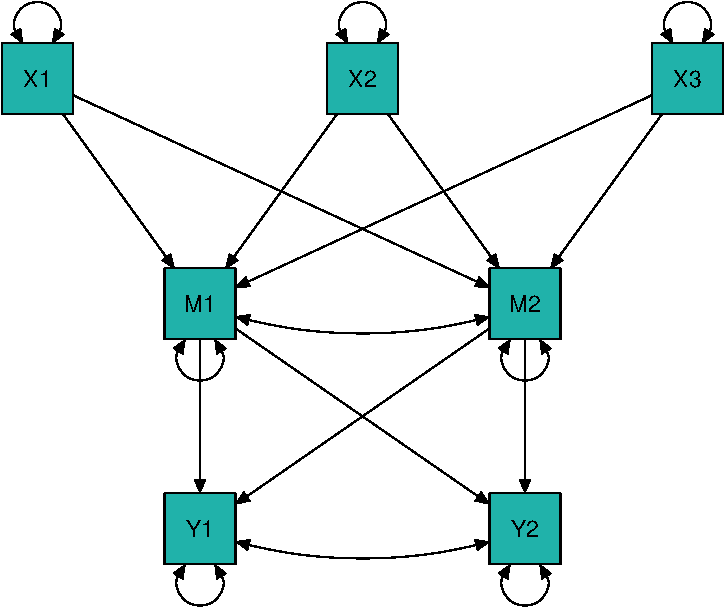
\includegraphics{Supplemental_materials_3_files/figure-latex/unnamed-chunk-14-1.pdf}

\begin{Shaded}
\begin{Highlighting}[]
\KeywordTok{sessionInfo}\NormalTok{()}
\end{Highlighting}
\end{Shaded}

\begin{verbatim}
## R version 3.5.1 (2018-07-02)
## Platform: x86_64-pc-linux-gnu (64-bit)
## Running under: Ubuntu 18.04 LTS
## 
## Matrix products: default
## BLAS: /usr/lib/x86_64-linux-gnu/blas/libblas.so.3.7.1
## LAPACK: /usr/lib/x86_64-linux-gnu/lapack/liblapack.so.3.7.1
## 
## locale:
##  [1] LC_CTYPE=en_US.utf8       LC_NUMERIC=C             
##  [3] LC_TIME=en_US.utf8        LC_COLLATE=en_US.utf8    
##  [5] LC_MONETARY=en_US.utf8    LC_MESSAGES=en_US.utf8   
##  [7] LC_PAPER=en_US.utf8       LC_NAME=C                
##  [9] LC_ADDRESS=C              LC_TELEPHONE=C           
## [11] LC_MEASUREMENT=en_US.utf8 LC_IDENTIFICATION=C      
## 
## attached base packages:
## [1] stats     graphics  grDevices utils     datasets  methods   base     
## 
## other attached packages:
## [1] metaSEM_1.1.1  OpenMx_2.9.9   knitr_1.20     semPlot_1.1   
## [5] lavaan_0.6-1   rmarkdown_1.10
## 
## loaded via a namespace (and not attached):
##   [1] nlme_3.1-137         RColorBrewer_1.1-2   rprojroot_1.3-2     
##   [4] mi_1.0               tools_3.5.1          backports_1.1.2     
##   [7] R6_2.2.2             d3Network_0.5.2.1    rpart_4.1-13        
##  [10] Hmisc_4.1-1          lazyeval_0.2.1       colorspace_1.3-2    
##  [13] nnet_7.3-12          tidyselect_0.2.4     gridExtra_2.3       
##  [16] mnormt_1.5-5         curl_3.2             compiler_3.5.1      
##  [19] qgraph_1.5           fdrtool_1.2.15       htmlTable_1.12      
##  [22] network_1.13.0.1     scales_0.5.0         checkmate_1.8.5     
##  [25] mvtnorm_1.0-8        psych_1.8.4          pbapply_1.3-4       
##  [28] sem_3.1-9            stringr_1.3.1        digest_0.6.15       
##  [31] pbivnorm_0.6.0       foreign_0.8-70       minqa_1.2.4         
##  [34] rio_0.5.10           base64enc_0.1-3      jpeg_0.1-8          
##  [37] pkgconfig_2.0.1      htmltools_0.3.6      lme4_1.1-17         
##  [40] lisrelToR_0.1.4      highr_0.7            htmlwidgets_1.2     
##  [43] rlang_0.2.1          readxl_1.1.0         huge_1.2.7          
##  [46] rstudioapi_0.7       bindr_0.1.1          gtools_3.8.1        
##  [49] statnet.common_4.1.4 acepack_1.4.1        dplyr_0.7.6         
##  [52] zip_1.0.0            car_3.0-0            magrittr_1.5        
##  [55] Formula_1.2-3        Matrix_1.2-14        Rcpp_0.12.17        
##  [58] munsell_0.5.0        abind_1.4-5          rockchalk_1.8.111   
##  [61] whisker_0.3-2        stringi_1.2.3        yaml_2.1.19         
##  [64] carData_3.0-1        MASS_7.3-50          plyr_1.8.4          
##  [67] matrixcalc_1.0-3     grid_3.5.1           parallel_3.5.1      
##  [70] forcats_0.3.0        lattice_0.20-35      haven_1.1.2         
##  [73] splines_3.5.1        hms_0.4.2            sna_2.4             
##  [76] pillar_1.2.3         igraph_1.2.1         rjson_0.2.20        
##  [79] boot_1.3-20          corpcor_1.6.9        BDgraph_2.51        
##  [82] reshape2_1.4.3       stats4_3.5.1         XML_3.98-1.11       
##  [85] glue_1.2.0           evaluate_0.10.1      latticeExtra_0.6-28 
##  [88] data.table_1.11.4    png_0.1-7            nloptr_1.0.4        
##  [91] cellranger_1.1.0     gtable_0.2.0         purrr_0.2.5         
##  [94] assertthat_0.2.0     ggplot2_3.0.0        openxlsx_4.1.0      
##  [97] semTools_0.5-0       coda_0.19-1          glasso_1.8          
## [100] survival_2.42-3      tibble_1.4.2         arm_1.10-1          
## [103] ggm_2.3              ellipse_0.4.1        bindrcpp_0.2.2      
## [106] cluster_2.0.7-1
\end{verbatim}


\end{document}
